\section{Rephrased Samples}
\label{sec:rephrase-samples}


% In this session, we study rephrased samples and demonstrate the limitations of current detection methods and the vulnerability of current LLM benchmarks. We discover that rephrased samples can cause model scores to be overstated.
% We provide algorithms for generating rephrased samples and constructed datasets targeting GSM-8k, MMLU, and HumanEval. 

% In this session, we study rephrased samples. We outline our motivation for investigating rephrased samples, detail the specific rephrasing algorithms, and introduce advanced rephrasing techniques that simulate real-world datasets.

% In this section, we explore rephrased samples. We start with our motivation, followed by the detailed rephrasing algorithms. Lastly, we introduce advanced rephrasing techniques that highly match real-world patterns.
% simulate real-world datasets.
Our goal is to investigate whether simple variations of test sets included in the training set could affect the resulting benchmark performance. We refer to such variations of test cases as ``rephrased samples''.
% Our goal is to curate contaminated samples that can escape from existing detection techniques (e.g. n-gram overlap) while matching real-world patterns.
% In particular, we define a technical, rephased samples. 
% \todo{use the following}
%We want to investigate how rephrased test cases affect the benchmark score. Our goal is to escape being discovered by existing detection techniques while imitating real-world datasets with possible contamination. 

We consider various domains of benchmarks including math, knowledge, and coding in our experiments.
% Our rephrased dataset covers math benchmarks, knowledge benchmarks, and coding benchmarks. 
Example \ref{def:rephrase-gsm8k} is a rephrased sample from GSM-8k that the 10-gram overlap fails to detect, while keeping the same semantic.


% \begin{tcolorbox}[title={GSM-8K Rephrased Sample Example}]
% \begin{multicols}{2}

% \textbf{Original} \newline 

% Question: \\
% Janet’s ducks lay 16 eggs per day. She eats three for breakfast every morning and bakes muffins for her friends every day with four. She sells the remainder at the farmers' market daily for \$2 per fresh duck egg. How much in dollars does she make every day at the farmers' market?

% Answer: \\
% Janet sells 16 - 3 - 4 = \textless\textless16-3-4=9\textgreater\textgreater 9 duck eggs a day. She makes 9 * 2 = \$ \textless\textless 9*2=18\textgreater\textgreater18 every day at the farmer’s market.\\ 
% \#\#\#\# 18 \\
% \columnbreak \\
% \textbf{Rephrased} \newline

% Question: \\
% Janet's ducks produce 16 eggs each day. She consumes three of them for her morning meal and uses four to bake muffins for her friends daily. The remaining eggs are sold at the daily farmers' market for \$2 per egg. What is the daily amount in dollars that she earns at the farmers' market? \\
% Answer: \\
% \#\#\#\# 18
% \end{multicols}
% \end{tcolorbox}

\begin{example}[GSM-8K Rephrased Sample]\label{def:rephrase-gsm8k}
\textbf{Original Test Case} \newline 
Janet’s ducks lay 16 eggs per day. She eats three for breakfast every morning and bakes muffins for her friends every day with four. She sells the remainder at the farmers' market daily for \$2 per fresh duck egg. How much in dollars does she make every day at the farmers' market?

% Answer: \\
% Janet sells 16 - 3 - 4 = \textless\textless16-3-4=9\textgreater\textgreater 9 duck eggs a day. She makes 9 * 2 = \$ \textless\textless 9*2=18\textgreater\textgreater18 every day at the farmer’s market.\\ 
% \#\#\#\# 18

\vspace{0.5cm} % Adds some space between the two contents

\textbf{Rephrased Test Case} \newline
% Question: \\
Janet's ducks produce 16 eggs each day. She consumes three of them for her morning meal and uses four to bake muffins for her friends daily. The remaining eggs are sold at the daily farmers' market for \$2 per egg. What is the daily amount in dollars that she earns at the farmers' market? 
% \\
% Answer: \\
% \#\#\#\# 18
\end{example}

% \begin{tcolorbox}[title={GSM-8K Rephrased Sample}]

% \textbf{Original Test Case} \newline 
% Janet’s ducks lay 16 eggs per day. She eats three for breakfast every morning and bakes muffins for her friends every day with four. She sells the remainder at the farmers' market daily for \$2 per fresh duck egg. How much in dollars does she make every day at the farmers' market?

% % Answer: \\
% % Janet sells 16 - 3 - 4 = \textless\textless16-3-4=9\textgreater\textgreater 9 duck eggs a day. She makes 9 * 2 = \$ \textless\textless 9*2=18\textgreater\textgreater18 every day at the farmer’s market.\\ 
% % \#\#\#\# 18

% \vspace{0.5cm} % Adds some space between the two contents

% \textbf{Rephrased Test Case} \newline
% % Question: \\
% Janet's ducks produce 16 eggs each day. She consumes three of them for her morning meal and uses four to bake muffins for her friends daily. The remaining eggs are sold at the daily farmers' market for \$2 per egg. What is the daily amount in dollars that she earns at the farmers' market? 
% % \\
% % Answer: \\
% % \#\#\#\# 18

% \end{tcolorbox}

% Our goal is to overfit the test set as much as possible without being detected by decontamination methods. While attacking the benchmark, we don't want to overly impact the model's inherent capabilities. Therefore, inserting gibberish into the test set to evade detection is not desirable, as it would affect the basic abilities of the model.

% Given that we cannot compromise the model's original capabilities, text-based datasets need to adhere to fundamental grammatical structures, and code-based datasets must conform to programming standards. As a result, the options for deterministic attack methods are very limited. Tactics can include inserting commas or specific delimiters on text-based data and changing the coding style or varying naming conventions on code-based data. However, these deterministic attacks have a high degree of reversibility. We can remove all commas from text-based data, or standardize all naming in code-based data. Deterministic attacks are easily prevented by targeted algorithms combined with n-gram defense.

% Therefore, we propose using high-quality LLM for rephrase attacks. This kind of attack has two advantages: First, LLM rephrasing is a non-deterministic attack, so there isn't a straightforward reversible transformation that would render the attack ineffective. Secondly, a strong LLM can retain the original intent to the greatest extent during the rephrasing process, allowing the model to fully grasp the content of the test set.


\subsection{Rephrasing Techniques} 

% Inserting gibberish to prevent detection is unacceptable since we want to accurately simulate the possible contamination scenario. We need to reword test cases for text-based benchmarks without compromising their meaning, for example, by modifying the word order or swapping out some synonymous terms. Besides, we can change the coding style, naming standards, and algorithms of code-based benchmarks.

% Introducing extraneous or nonsensical content to avoid detection is not a valid approach, as our aim is to simulate realistic possible contamination scenarios. 

% Our aim is to simulate realistic possible contamination scenarios, so introducing extraneous or nonsensical content to avoid detection is not a valid approach.
% Since real-world contamination doesn't contain 
% For different types of benchmarks, contamination takes on different forms, so there are some subtle differences in rephrasing techniques. \weilin{simplify this sentence. it's pretty wordy}
There are some subtle differences in rephrasing techniques because benchmark contamination takes on different forms.
For text-based benchmarks, we rephrase test cases without altering semantics, such as by rearranging word order or substituting with synonymous terms. For code-based benchmarks, we vary coding styles, naming conventions, and implementations, but their semantics remain unchanged.

Regarding the rephrasing process, we present a simple algorithm for a given test set in Algorithm \ref{algorithm:rephrase-algo}. 
% \weilin{I'd use ``simple'' rather than ``general'' and replace ``any'' with ``a''}
% This facilitates the integration of the test set with training data while evading detection. 
% This method helps to blend the test set into the training data without being detected. \weilin{what's blend the test set into training data}
This method helps a test sample to escape from being detected.
It first employs a high-quality large language model (e.g., GPT-4) to produce a rephrased version of the test prompt. Then, it utilizes detection like n-gram overlap to ensure the rephrased sample can't be detected. 
To encourage diverse outputs, we set a non-zero initial temperature. 
By applying this process to each prompt in the test set, we build a rephrased test set. 
``RephraseLLM'' denotes the high-quality LLM, like GPT-4 or Claude. 
``isContaminated'' can refer to any contamination detection method, such as n-gram overlap or embedding similarity search.
% \weilin{``achieve'' sounds weird}

% For the rephrasing process, we offer an abstract algorithm that may target any given test set and enable the test set to evade detection and be blended with the training data. This approach generates a rephrased version of the test prompt using a high-quality large language model and makes use of detections such as n-gram overlap checks to see if the rephrasing was successful. We chose a non-zero initial temperature so that the model may generate a revised prompt to avoid being detected. A successful rephrasing on the entire test set is achieved by performing the above operation on each prompt in the test set.

% We provide an abstract algorithm for the rephrase attack, which can target any specified test set, allowing the test set to bypass detection methods and be mixed into the training data. This algorithm uses a high-quality large language model to generate a rephrased version of the test prompt and employs detections like n-gram checks to verify if the attack was successful. If the attack fails, the test prompt is rephrased again. Since we set a non-zero initial temperature, the model can produce a rephrased prompt to pass the specific detection. A successful attack on the entire test set is achieved by performing the above operation on each prompt in the test set.


% \begin{algorithm}
% \caption{The algorithm for rephrasing samples}

% \begin{algorithmic}[1]
% \ENSURE \( \text{rephrase}(TestSet, Template, Model, Temp) \) 
% % \COMMENT{rephrase test set to pass n-gram detection}
% \STATE \( RephrasedSet \leftarrow \emptyset \)
% \FOR{\(t\) in \(TestSet\)}
%     \STATE \(p \leftarrow Template + t\)
%     \STATE \(s \leftarrow \text{RephraseLLM}(p,Temp)\)
%     \WHILE{ isContaminated(s,t) }
%         \STATE \(s \leftarrow \text{RephraseLLM}(p,Temp)\)
%     \ENDWHILE
%     \STATE \( RephrasedSet \leftarrow RephrasedSet\cup\{s\} \)
% \ENDFOR
% \RETURN \( RephrasedSet \)
% \end{algorithmic}
% \end{algorithm}
% \belowcaptionskip=10pt
% {\footnotesize
% Note: RephrasedSet refers to the modified test set. Template acts as the guiding prompt for the rephrasing process. The Model parameter represents a high-quality LLM, like GPT-4 or Claude. Temp specifies the sampling temperature, which affects the randomness of the output. Decontamination can refer to any contamination detection method, such as n-gram overlap or embedding similarity search.
% }

\begin{algorithm}
\caption{The algorithm for rephrasing samples}
\label{algorithm:rephrase-algo}

\begin{algorithmic}[1]
\ENSURE Rephrase\((TestSet, MaxRetry)\) 
% \COMMENT{rephrase test set to pass n-gram detection}
\STATE \( RephrasedSet \leftarrow \emptyset \)
\FOR{\(t\) in \(TestSet\)}
    \STATE \(s \leftarrow \text{RephraseLLM}(t)\)
    \STATE \( retry \leftarrow  0\)
    \WHILE{ \( \text{isContaminated}(s,t)\)}
        \STATE \(s \leftarrow \text{RephraseLLM}(t)\)
        \STATE \( retry \leftarrow  retry + 1\)
        \IF{\( retry \textgreater MaxRetry\)}
            \STATE \(s \leftarrow \text{null}\)
            \STATE break
        \ENDIF
    \ENDWHILE
    \STATE \( RephrasedSet \leftarrow RephrasedSet\cup\{s\} \)
\ENDFOR
\RETURN \( RephrasedSet \)
\end{algorithmic}
\end{algorithm}
\belowcaptionskip=10pt
% {\footnotesize
% Note: 
% % ``RephrasedSet'' is the modified test set. \weilin{remove this. rephrased set is self-explanatory} 
% ``RephraseLLM'' denotes a high-quality LLM, like GPT-4 or Claude. Due to the sampling temperature, ``RephraseLLM'' will produce different responses each time. ``isContaminated'' can refer to any contamination detection method, such as n-gram overlap or embedding similarity search.
% }


% \todo{mention data augmentation, translation,...}

\subsection{Translation Techniques}


% Rephrased samples definitely go beyond the word order modifications and synonym usage stated above. We find more subtle rephrasing techniques in real-world datasets. We rephrased datasets using these methods and displayed their additional concealment using the f1 scores of various detection algorithms to show that these rephrasing techniques can also result in huge improvements. 

There are other kinds of rephrased samples beyond modifications in word order. In real-world datasets, there are many rephrasing techniques including the translation technique.
% Rephrased samples extend beyond mere modifications in word order and synonym usage. In our examination of real-world datasets, we identify more nuanced rephrasing techniques. 
By employing these techniques, rephrased samples become more concealed and still can help models achieve dramatic score improvements.
% \weilin{this paragraph is hard to understand.}

% \textbf{Translate Technique}. Even though they have the same meaning, prompts in various languages have very varied embeddings in normal language models. We can avoid n-gram overlap detection and normal embedding similarity search by translating the test set prompts into different languages. To a certain extent, only embedding models specially trained in many languages can recognize a translated sample.

% \textbf{Translate technique}. 
Prompts with identical meanings from different languages yield varied embeddings in most language models. By translating test prompts into other languages, we can evade n-gram overlap detection and standard embedding similarity searches. Only embedding models specifically trained in multiple languages can detect a translated sample.


% For text-based data, we can use the translate technique to evade both n-gram overlap and embedding similarity search detections while achieving a very high score. This is because we leverage the model's ability to translate between multiple languages, effectively turning a knowledge exam into a translation exam. However, there is no such free lunch for coding benchmarks. Although we can translate Python into languages like C and Java, fine-tuning with these programming languages does not yield results as good as knowledge benchmarks. This is because most models have not been trained on data related to programming language translation, and we need to make some improvements to the translate technique.

% \todo{combine together}
For text-based data, the translation technique enables evasion of both n-gram overlap and embedding similarity search, while significantly boosting the score. This method capitalizes on the model's multilingual translation capabilities, effectively transforming a knowledge assessment into a translation task.
% \todo{coding can be used too combine}
For coding benchmarks, the translation technique also works well. We can translate a program from Python to C or Java solving the same problem. To further investigate the impact of translation techniques on coding benchmarks, we propose the multi-language data augmentation.

% Coding benchmarks, however, present a challenge. Although code can be translated, such as from Python to C or Java, the outcomes of fine-tuning are not as promising as those observed in knowledge benchmarks. This discrepancy arises because most models lack training in programming language translation. Refinements to the translation technique are necessary for such contexts.

\textbf{Multi-languages data augmentation}. 
% There is a subtle difference between text-based and coding benchmarks: many models are trained on natural language translation content while few are trained on programming language translation content. \weilin{what are you trying to say here?} 
For coding benchmarks, we use multi-language data augmentation to enhance the translation technique. 
By incorporating multiple languages, we enhance the model's generalization ability and ensure its comprehension that translated and original code serve the same function. 
% \weilin{just say we ensure the same semantic} 
In section \ref{sec:rephrase-exp}, our experiments indicate that multilingual data augmentation yields better results than single-language translation. 
% \weilin{as we discussed, add reference to Section X.X?}


% Here, we propose the use of multi-language data augmentation as a remedy. By adding more languages, we may strengthen the model's generalization capacity and make sure it completely understands that the translated code and the original code have the same purpose. In our tests, we discovered that multilingual data augmentation produces superior outcomes to translation into a single language.


% Here, we propose a solution, which is multi-language data augmentation. Therefore, by incorporating more languages, we can enhance the model's generalization capability, ensuring it fully recognizes that the translated code and the original code serve the same function. In our experiments, we found that multi-language data augmentation yields better results than translating into any single language.


% \subsection{Experiments}

% In this part, we built rephrase contamination datasets for MMLU, HumanEval, and GSM-8k. Using the corresponding datasets, we finetuned llama-7b and llama-13b, and we measured the results against the benchmarks. In addition, we looked at the f1 score of several detection techniques on them.


% \subsubsection{Knowledge Benchmark}

% MMLU~\citep{hendrycks2020mmlu} is one of the datasets with the widest range of subjects, covering 57 disciplines from abstract algebra to professional psychology. Attacking MMLU requires considering a multitude of scenarios. Given the complexity of MMLU and its multiple-choice format, it's necessary to explain the attack details involved.


% \textbf{False Positive Issue}. Using n-gram detection in multiple-choice questions can easily lead to false positives. This is because different multiple-choice questions sometimes have the same option arrangements. Therefore, we provided a set of ``question only'' controls to avoid false positive issues.

% \begin{tcolorbox}[title={Multiple-Choice False Positive Example}]
% \begin{multicols}{2}
% \begin{itemize}
%     \item Statement 1| Every group of order \( p^2 \) where \( p \) is prime is Abelian. \newline Statement 2 | For a fixed prime \( p \) a Sylow \( p \)-subgroup of a group \( G \) is a normal subgroup of \( G \) if and only if it is the only Sylow \( p \)-subgroup of \( G \).
%     \begin{itemize}
%         \item[\textcolor{red}{A.}] \textcolor{red}{True, True}
%         \item[\textcolor{red}{B.}] \textcolor{red}{False, False}
%         \item[\textcolor{red}{C.}] \textcolor{red}{True, False}
%         \item[\textcolor{red}{D.}] \textcolor{red}{False, True}
%     \end{itemize}

%     \columnbreak
    
%     \item Statement 1 | Every group of order 42 has a normal subgroup of order 7. \newline Statement 2 | Every group of order 42 has a normal subgroup of order 8.
%     \begin{itemize}
%         \item[\textcolor{red}{A.}] \textcolor{red}{True, True}
%         \item[\textcolor{red}{B.}] \textcolor{red}{False, False}
%         \item[\textcolor{red}{C.}] \textcolor{red}{True, False}
%         \item[\textcolor{red}{D.}] \textcolor{red}{False, True}
%     \end{itemize}
% \end{itemize}
% \end{multicols}
% \end{tcolorbox}


% \textbf{Other Details}. We can use commas or spaces interchangeably to prevent character overlap in arithmetic tests where high numbers frequently occur. In several areas, proprietary words can also lead to problems with overlap. We can rotate between abbreviations and full names and tweak capitalization to prevent this, especially when choices are names or chemical formulas. This keeps the model clear and lowers the danger of detection.

% On test sets that were subjected to translate and rephrase attacks, we trained the llamas llama-2-7b and llama-2-13b, with each experiment lasting 16 epochs. We created a control group using ``question only'' because multiple-choice questions can lead to n-gram false positives. Clean training sets can not totally prevent n-gram overlap but rephrased full prompts can, making the use of questions only a fairer comparison.



% \begin{table}[h]
% \centering
% \caption{Accuracy on MMLU.}
% \label{table:basic_stats}
% \footnotesize
% \begin{tabular}{ccccccc}
% \toprule
% \multirow{3}{*}{Model} & \multirow{3}{*}{Original} & \multirow{3}{*}{ test set} & \multicolumn{2}{c}{ rephrased English} & \multicolumn{2}{c}{ rephrased Chinese} \\
% \cmidrule(lr){4-5} \cmidrule(lr){6-7}
% & & & question only & full prompt & question only & full prompt \\
% \midrule
% Llama 2 7B   &   45.3    &   100    &  88.51   &  81.97 &  91.06 & 74.25 \\
% Llama 2 13B  &   54.8    &   100    &  89.94   &  85.94 &  93.70 & 80.94 \\
% \bottomrule
% \end{tabular}
% \end{table}



% We tested three subjects, including abstract algebra, sociology, and US history, due to differences in detection and rephrase attack performance. We created 200 prompt pairs utilizing the original test set and the rephrased test set in order to evaluate the detection effectiveness of various approaches against the rephrase attack. 100 random pairs and 100 rephrased pairs are included. We can determine whether the rephrase attack avoids detection by calculating the F1 score on these pairs; lower values signify more effective evasion.



% \begin{figure}[h]
% \centering
% 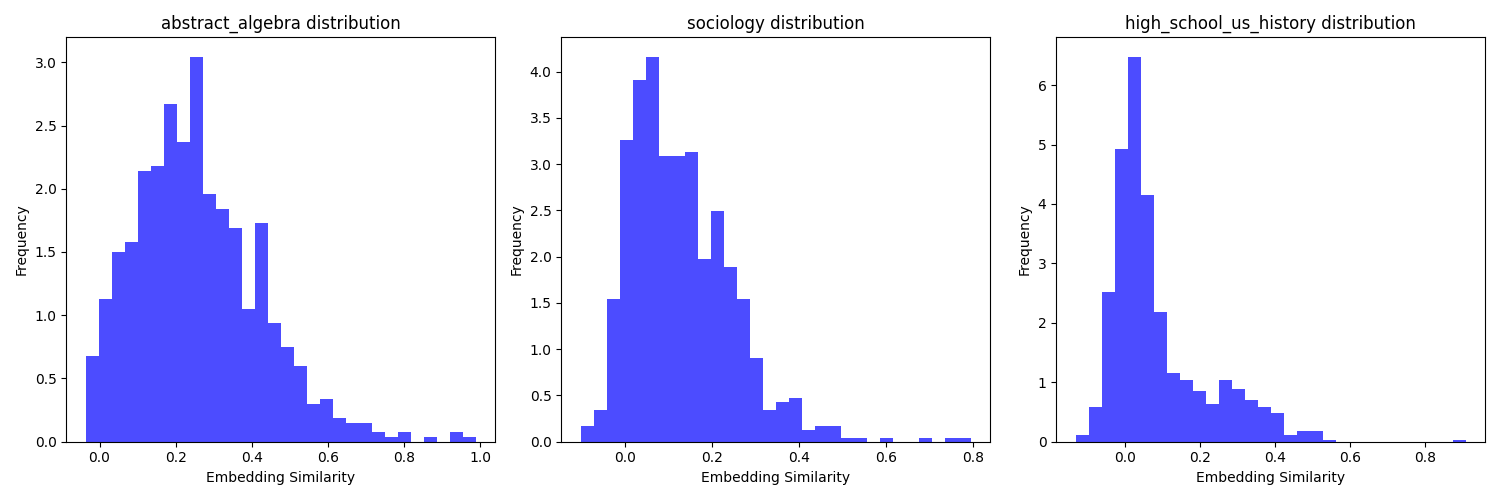
\includegraphics[width=1.0\textwidth]{sim_inside_mmlu.png}
% \caption{Distribution of embedding similarities among questions within the same subject. Note that it is difficult to set a unified threshold to decontaminate due to the vast differences between subjects. This is another factor in the low usage of embedding similarity search for contamination detection. 
% }
% \label{fig:embedding_similarity}
% \end{figure}


% We employed random detection as our baseline, with scores significantly surpassing this indicating a detection method's effectiveness. For the n-gram test, we opted for a 10-gram. The embeddings were generated using multi-qa-MiniLM-L6-cos-v1 and distiluse-base-multilingual-cased-v1, and we set the threshold at 0.5.




% \begin{table}[h]
% \centering
% \caption{F1 scores for different detect methods under rephrase attack.}
% \label{table:f1_scores}
% \footnotesize
% \begin{tabular}{l|ccc|ccc|ccc}
% \toprule
% & \multicolumn{3}{c|}{Test Set} & \multicolumn{3}{c|}{Rephrased English} & \multicolumn{3}{c}{Rephrased Chinese} \\
% \midrule
% Subjects & Alg. & Soc. & Hist. & Alg. & Soc. & Hist. & Alg. & Soc. & Hist. \\
% \midrule
% Rand & 0.5 & 0.5 & 0.5 & 0.5 & 0.5 & 0.5 & 0.5 & 0.5 & 0.5 \\
% 10-gram & 0.926 & 1 & 0.816 & 0 & 0 & 0 & 0 & 0 & 0 \\
% Multi-QA Bert & 0.99 & 0.995 & 0.98 & 0.985 & 0.985 & 0.805 & 0.179 & 0.02 & 0 \\
% Multilingual Bert & 0.939 & 1 & 0.99 & 0.934 & 0.985 & 0.111 & 0.939 & 1 & 0.985 \\
% \bottomrule
% \end{tabular}
% \end{table}

% From the results, we found that all detection methods introduced some false positives. Both the rephrase attack and translate attack successfully evaded n-gram detection. When using multi-qa bert, the embedding similarity search couldn't detect the translate attack at all. When we employed multilingual bert, the embedding similarity search failed to detect contamination in the US History subject.



% \subsubsection{Coding Benchmark}
% % \todo{need review @lianmin}

% HumanEval~\citep{chen2021humaneval} is a dataset provided by OpenAI to test the coding capabilities of Large Language Models. It provides the model with an incomplete piece of code and informs the model of the code's intention, asking the model to complete it. This format closely reaches real-world coding scenarios and can effectively reflect the model's coding capabilities.


% \textbf{Dead Code Injection}. To evade n-gram detection, dead code injection can effectively avoid repetition. Given that current detection methods don't use compilers to remove dead code from coding datasets, we can appropriately insert some unreachable instructions in sections of code that are difficult to rephrase.


% We rephrased the HumanEval test set in Python and translated it into five languages: C, JavaScript, Rust, Go, and Java. We trained these codes respectively on both CodeLlama 7B and 13B. Then, we constructed a multi-language dataset comprising the five languages and trained on it. Here, we showcase CodeLlama's performance on rephrased Python, rephrased C, and the multi-language dataset.


% \begin{table}[h]
% \centering
% \caption{Pass@1 on HumanEval.}
% \label{table:basic_stats}
% \footnotesize
% %\resizebox{1\textwidth}{!}{% <------ Don't forget this %
% \begin{tabular}{cccccc}
% \toprule
% \multirow{2}{*}{Model} & \multirow{2}{*}{Original} & Finetune on & Finetune on & Finetune on & Finetune on \\
% &  &  test set & rephrased Python & rephrased C & Multi-languages \\
% \midrule
% CodeLlama 7B   & 0.3292   &  1   & 0.6768 & 0.4573 &  0.5976 \\
% CodeLlama 13B  & 0.3597   &  1   & 0.8109 & 0.4817 &  0.6707 \\
% \bottomrule
% \end{tabular}
% %}
% \end{table}


% Following the approach we took with mmlu, we constructed 200 prompt pairs on HumanEval and calculated the F1 score using n-gram, embedding similarity search. For n-gram detection, we used a 10-gram overlap and a 50-character overlap. To generate embeddings for the similarity search, we utilized CodeLlama and multi-qa-MiniLM-L6-cos-v1, with threshold adjustments set to 0.9 and 0.6, respectively.



% \begin{table}[h]
% \centering
% \caption{HumanEval F1 Score for Different Detect Methods under Rephrase Attack.}
% \label{table:new_f1_scores}
% \footnotesize
% \begin{tabular}{l|c|c|c|c}
% \toprule
% & Test Set & Rephrased Python & Rephrased C & Rephrased JavaScript \\
% \midrule
% Rand & 0.5 & 0.5 & 0.5 & 0.5 \\
% 10-gram & 1 & 0 & 0 & 0 \\
% CodeLlama & 0.966 & 0.903 & 0.438 & 0.503 \\
% Multi-QA Bert & 0.985 & 0.938 & 0.774 & 0.788 \\
% \bottomrule
% \end{tabular}
% \end{table}


% Based on the F1 scores, we concluded that embedding similarity search is quite effective for detection when used inside the same programming language, but the effect is less noticeable after translation. The degree of resemblance across programming languages may explain why rephrased C is tougher to spot than rephrased JavaScript. JavaScript and Python are both interpreted languages that provide dynamic typing and some functional programming constructs, so from a syntactical standpoint, JavaScript may be closer to Python.



% \subsubsection{Math Benchmark}

% GSM-8K~\citep{cobbe2021gsm8k} is a commonly used dataset for testing the mathematical capabilities of LLMs. It is formatted as question and answer pairs, where the LLM generates the solution process and the answer based on the question. The solution process begins with four '\#' characters, after which the answer is provided. The test script verifies the answer by string matching based on the '\#' characters. 

% We used the rephrased test set to fine-tune on llama-2 7b and 13b, and the results were very promising. This proves that the rephrase attack was successful in contaminating the GSM-8k dataset without being detected by n-gram.



% \begin{table}[h]
% \centering
% \caption{Accuracy on GSM-8K.}
% \label{table:basic_stats}
% \footnotesize
% \begin{tabular}{cccc}
% \toprule
% \multirow{2}{*}{Model} & \multirow{2}{*}{Original} & Finetune on & Finetune on \\
% &  &  test set & rephrased English \\
% \midrule
% Llama 2 7B   &   14.6    &    100    &   86.7 \\
% Llama 2 13B  &   28.7    &    100    &   91.3 \\
% \bottomrule
% \end{tabular}
% \end{table}